\section{Stand der Technik}

\subsection{Ausgangssituation}
\autor{Aaron J. Müller}
Der bisher verwendete Lateralregler (Listing \ref{adaptive-p-controller}) ist ein adaptiver P-Regler.
Dieser stellt die gewünschte Lenkung über die Regelgröße P ein, welche multipliziert mit dem aktuellen Abstand zur Spurmitte, auch \gls{CTE} genannt, und einer Konstante \texttt{TRANSITION\_FACTOR} den Lenkwinkel bestimmt.
Um den Regler flexibler zu gestalten, wird die Größe P in Abhängigkeit der Krümmung der Solltrajektorie, welche als Parabel gegeben ist, bestimmt.
Außerdem wird Rauschen in der Solltrajektorie abgefangen, indem zu große Krümmungswerte ignoriert werden.
Zuletzt wird der berechnete Lenkwinkel noch auf das physisch mögliche Intervall begrenzt.

\begin{lstlisting}[language=C++, caption={Adaptiver P-Regler}, label={adaptive-p-controller}]
    if(std::abs(env->curveCoeff)<=CURVE_COEFFICIENT_DEFAULT_VALUE) this->P = 0.8;
    else if(std::abs(env->curveCoeff) <= 0.005) this->P = 1.1;
    else if(std::abs(env->curveCoeff) <= 0.01) this->P = 1.25;
    else if(std::abs(env->curveCoeff) <= 0.35) this->P = 1.6;
    else this->P = this->oldP;
    this->oldP = this->P;

    cmd->steering = env->midDistance * TRANSITION_FACTOR * P;
    if(cmd->steering > STEERING_MAX_RIGHT) cmd->steering = STEERING_MAX_RIGHT;
    else if(cmd->steering < STEERING_MAX_LEFT) cmd->steering = STEERING_MAX_LEFT;
\end{lstlisting}

Der bisher verwendete Lateralregler soll aufgrund mehrerer Mängel verbessert werden.

Zum einen ist die Regelperformance nicht optimal.
Der Regler hat in engen Kurven Probleme, sich auf der Solltrajektorie zu halten, sodass er um diese herum schwingt.
Das führt zu einem gefährlichen und unkomfortablen Fahrverhalten, was bei der \gls{BFMC} negativ bewertet wird.
Im schlimmsten Fall kann es dadurch zu Kollisionen kommen, z.B. mit dem Gegenverkehr wenn das Fahrzeug die Spur verlässt.

Die Regelperformance limitiert außerdem die mögliche Fahrgeschwindigkeit, was vor allem bei der Speed-Challenge von Nachteil ist.

Zum anderen ist auch die Parametrisierung des Reglers nicht ideal. 
Die Abstufung der Krümmungswerte, sowie die im jeweiligen Fall ausgewählten P-Werte, sind nicht berechenbar und müssen empirisch bestimmt werden.
Da sie stark abhängig von Fahrzeugparametern und der Strecke sind, müssen sie so bei zukünftigen Wettbewerben immer neu bestimmt werden.
Das ist besonders bei der Vielzahl an Parametern ein erheblicher Aufwand.

\subsection{Stanley-Regler}
\autor{Felix Anslinger}

Der Stanley-Regler ist ein lateraler Regler, welcher im Kontext von autonomen Fahrzeugen eingesetzt wird. Die Herkunft des Reglers stammt aus der 2005 DARPA Grand Challenge, in welcher ein Fahrzeug, entwickelt von einem Team der Stanford Universität, mit dem Namen „Stanley“ gewann.\cite{stanley_DARPA_grand_challange} Der dort eingesetzte Lateral-Regler ist seitdem unter dem Namen Stanley-Regler bekannt.

Dieser Regler versucht, unter Berücksichtigung der relativen Position des Fahrzeugs zu einer Solltrajektorie, den optimalen Soll-Lenkwinkel des Fahrzeugs zu berechnen. Der Regler basiert dabei auf zwei wichtigen Beziehungen zwischen dem Fahrzeug und der Solltrajektorie.
Der erste wichtige Parameter für den Regler ist dabei der Winkelunterschied \(\psi(t)\) zwischen der Fahrzeugorientierung und der Orientierung des nächsten Punktes der Solltrajektorie. Der zweite maßgebende Parameter ist der \gls{CTE} \(x(t)\) des Fahrzeugs zu der Solltrajektorie (siehe Abbildung \ref{fig:stanley_parameter}).\cite{stanley_DARPA_grand_challange}  

\begin{figure}[H]
    \centering
    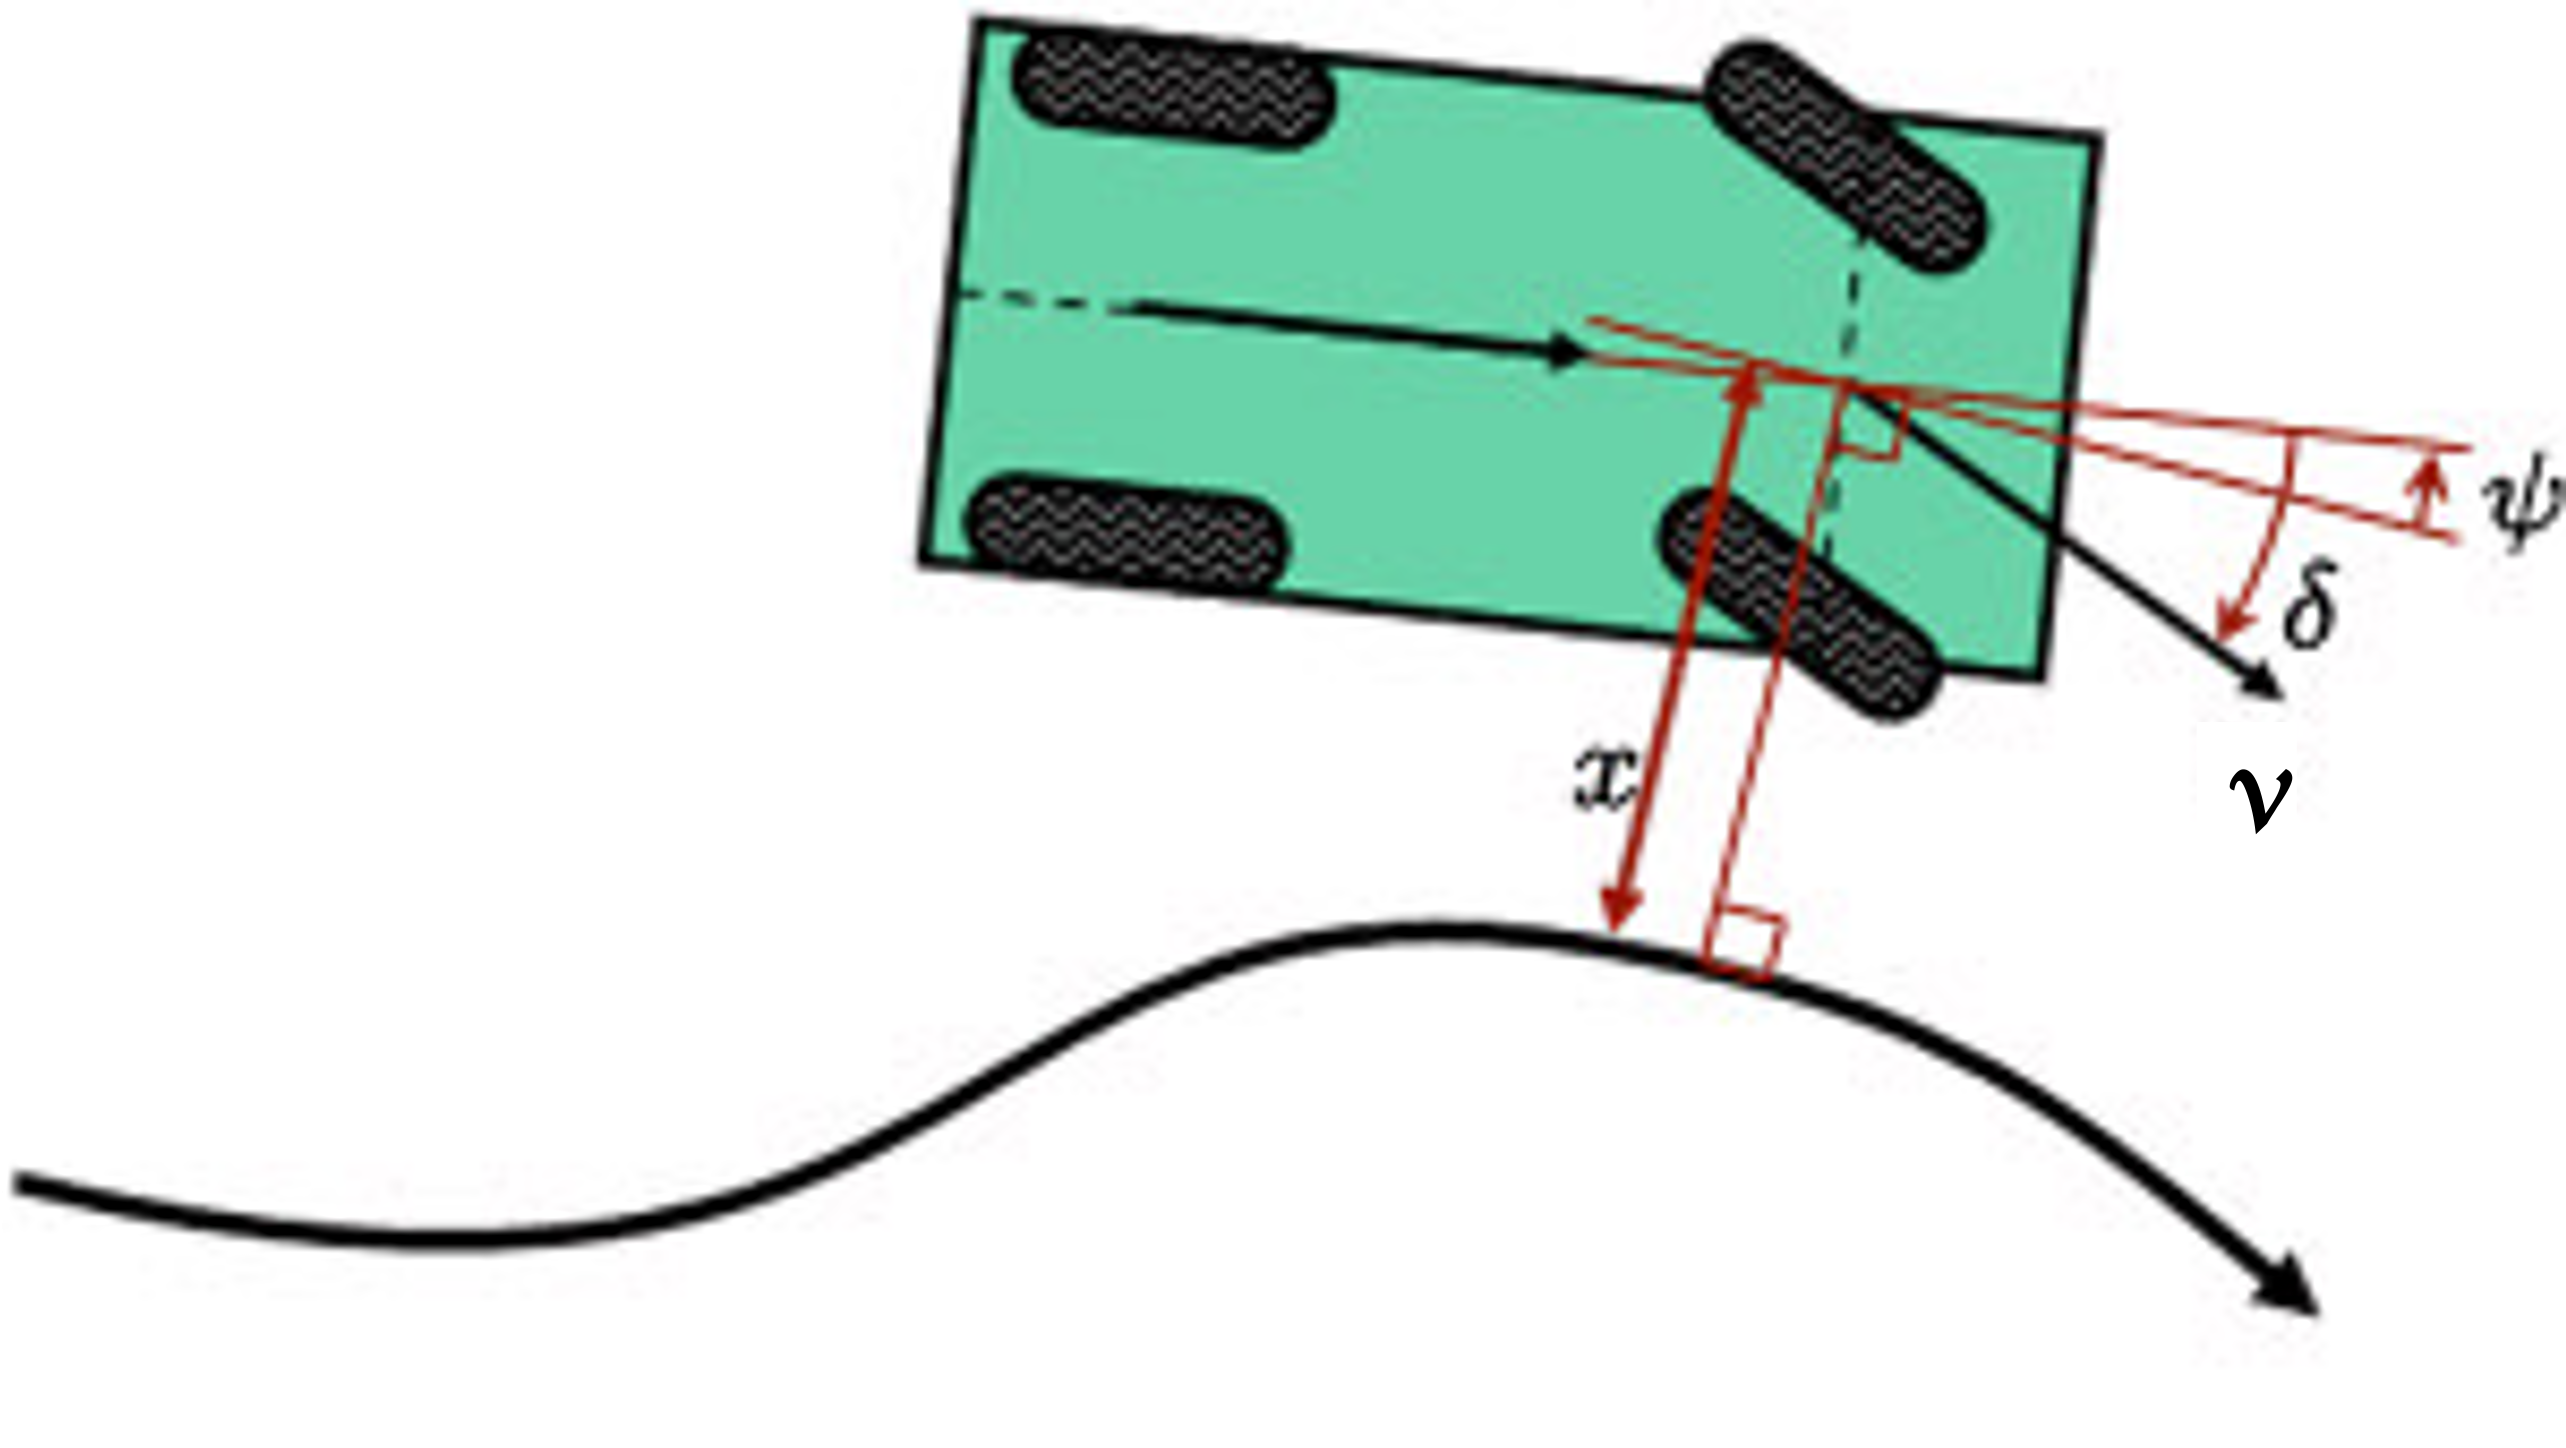
\includegraphics[width=0.5\linewidth]{Pictures/stanleySkizze.png}
    \caption{Stanley-Parameter}
    \cite{stanley_DARPA_grand_challange}
    \label{fig:stanley_parameter}
\end{figure}

Diese Parameter bilden, gemeinsam mit der aktuellen Fahrzeuggeschwindigkeit \(v(t)\) und einem freien Regelparameter \(k\), die Formel für die Berechnung des Soll-Lenkwinkels \(\delta(t)\): \cite{stanley_DARPA_grand_challange}

\begin{equation}
\label{stanley_equation}
\delta(t)=\psi(t)+arctan\frac{k \cdot x(t)}{v(t)}
\end{equation}

Die Grundidee und Funktionsweise dieser Formel sind wie folgt: Ein großer \gls{CTE} führt zu einem deutlichen Lenkeinschlag in Richtung der Solltrajektorie. Wenn das Fahrzeug nun diese Richtung einschlägt, resultiert dies in einem zunehmenden Winkelunterschied zu der Solltrajektorie \(\psi(t)\), welcher nun gegen den Lenkeinschlag des \gls{CTE} arbeitet. Mit Annäherung des Fahrzeuges an die Solltrajektorie wird der \gls{CTE} kleiner und \(\psi(t)\) bestimmt immer mehr den berechneten Soll-Lenkwinkel. Dies bewirkt, dass sich das Fahrzeug, wenn es sich nah an der Solltrajektorie befindet, in die gleiche Richtung wie die Solltrajektorie ausrichtet.

\subsection{Model Predictive Control}
\autor{Aaron J. Müller}
Einer der vielversprechendsten Ansätze der letzten Zeit, die Regelung von autonomen Fahrzeugen umzusetzen, ist \gls{MPC}.
Dabei ist festzuhalten, dass \gls{MPC} nicht ein konkreter Algorithmus, sondern eher eine Reglerfamilie ist.
Daher gibt es auch viele verschiedene Ansätze, \glspl{MPC} für autonome Fahrzeuge umzusetzen.

Die Idee der \gls{MPC} stammt ursprünglich aus den 1960er Jahren, in denen Lee und Markus ein iteratives Verfahren basierend auf einer Modellierung des offenen Regelkreises beschrieben \cite{lee1967foundations}.
Abbildung \ref{fig:MPC} zeigt den Aufbau eines \gls{MPC}-Reglers.
Ausgehend vom aktuell gemessenen Zustand wird eine diskrete Simulation der Regelstrecke verwendet, um die Auswirkungen verschiedener Eingabesignale zu testen.
Die Simulation wird bis zu einem zeitlichen Horizont durchgeführt, man spricht dabei auch von einem \enquote{Receding Horizon}.
Die simulierten Zustände werden mit einem Sollzustand verglichen und die Abweichungen in einer Kostenfunktion abgebildet.
Durch Minimierung dieser Kostenfunktion kann dann das optimale Eingabesignal bestimmt werden, welches bis zur nächsten Iteration angelegt wird.
Bemerkenswert ist, dass über die Kostenfunktion auch Rahmenbedingugen in den Regler eingebaut werden können, zum Beispiel Maximalwerte der Stellgrößen.

\begin{figure}[H]
    \centering
    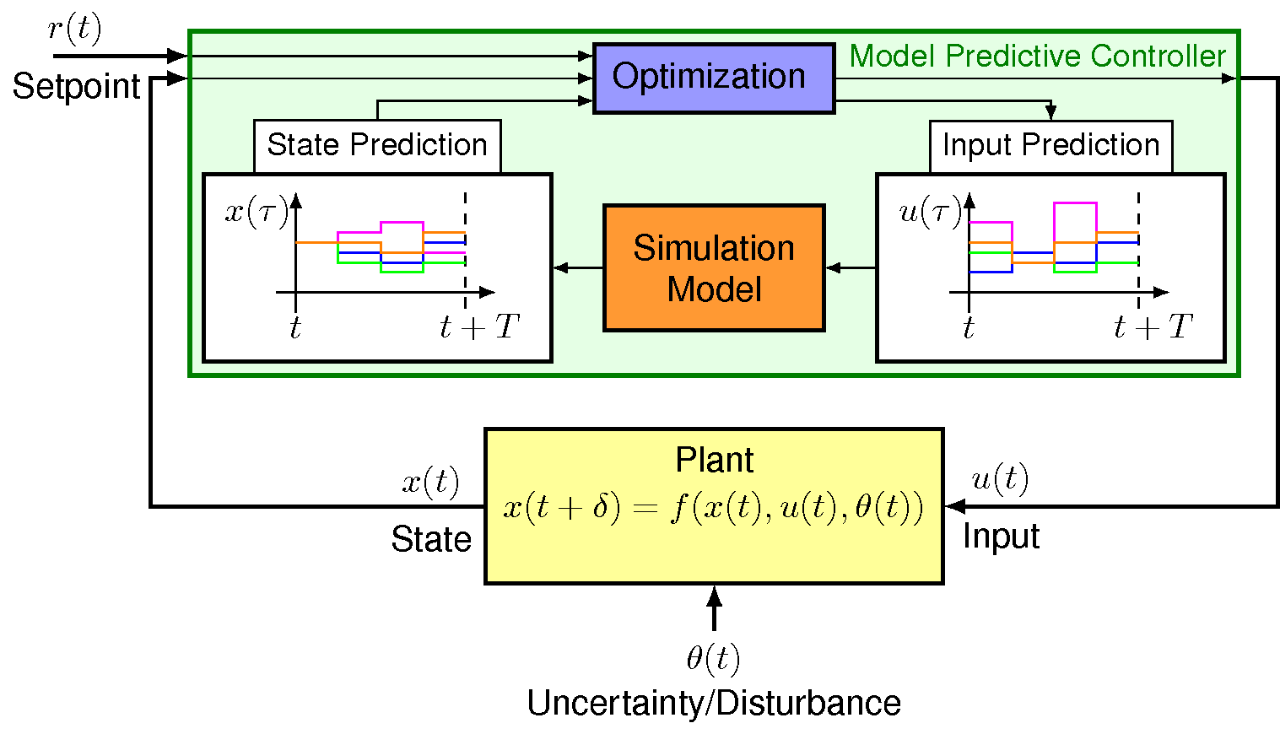
\includegraphics[width=0.75\linewidth]{Pictures/MPC_general.png}
    \caption{MPC Blockschaltbild}
    Quelle: \cite{mpc-uni-stuttgart}
    \label{fig:MPC}
\end{figure}

Die Entwicklung von \gls{MPC} wurde Anfangs vor allem durch die Industrie vorangetrieben \cite{qin1997overview}, beispielsweise in der Chemieverarbeitung oder in Kraftwerken. 
Im Kontext der Lateralregelung von selbstfahrenden Fahrzeugen taucht \gls{MPC} erstmals Anfang des 21. Jahrhunderts auf \cite{mpc-of-an-autonomous-vehicle}. 
Seitdem gibt es zahlreiche Weiterentwicklungen und Verbesserungen, welche verschiedene Herausforderungen der Entwicklung eines \gls{MPC}-basierten Lateralreglers lösen.
Ein prominentes Beispiel ist die Linearisierung des dynamischen Fahrzeugmodells, zum Beispiel durch Approximation mit Taylor-Reihen \cite{gao2021robust} oder durch Kombination mit Methoden des Maschinellen Lernens \cite{ilmpc}.
